\documentclass[twoside,12pt]{report}
\usepackage{thesis-style}	%Egyedi stílus
%\usepackage{sectsty}
\usepackage{lipsum}		%vakszöveg tesztelésre


%\addbibresource{bib/bibliography.bib}

\graphicspath{ {./fig/} }

\def\registeredlogo{\textsuperscript{\textregistered}}
\interfootnotelinepenalty=10000
%\setcounter{tocdepth}{1} % Show sections
%\setcounter{tocdepth}{2} % + subsections
\setcounter{tocdepth}{3} % + subsubsections
%\setcounter{tocdepth}{4} % + paragraphs
%\setcounter{tocdepth}{5} % + subparagraphs

% Töltsd ki a saját szakdolgozatod adataival
\def\CIM{Hibrid fordítás HPC környezetben}
%Új cím: Modern eszközök Deep Learning alkalmazások fejlesztéséhez
\def\SZERZO{Palkovics Dénes}
\def\SZAK{mérnökinformatikus BSc}
\def\VEDESEVE{2019}

\def\EGYETEM{Debreceni Egyetem}
\def\KAR{Informatikai Kar}
\def\TANSZEK{Komputergrafika és Képfeldolgozás Tanszék}
\def\TEMAVEZETO{Dr Kovács László}
\def\TEMAVEZETOBEOSZTAS{adjunktus}


\title{\CIM}
\author{\SZERZO}
\date{\VEDESEVE}

%\renewcommand{\familydefault}{\sfdefault}	%betűcsalád beállítása az egész dokumentumra

\begin{document}
%\cite{*} % az összes bejegyzés kiírása az irodalomjegyzékben
\pagenumbering{Roman}
\pagestyle{empty} 

\vspace*{0.2\paperheight}
{\sffamily
\begin{center}
{\Huge \textsc{Szakdolgozat}}
\end{center}
%\vfill
%\\[0.667\textheight]
\vspace{0.3\paperheight}
\begin{flushright}
	\SZERZO
\end{flushright}
\vfill
\begin{center}
	Debrecen\\
	\VEDESEVE
\end{center}
}
\cleardoublepage
% belső fedőlap
\begin{titlepage}
\begin{center}
\EGYETEM \\
\KAR \\
%\TANSZEK
\end{center}

\vfill

\begin{center}
\LARGE
\textbf{\CIM}
\normalsize
\end{center}

\vfill

\begin{minipage}[lt]{0.45\linewidth}
\centering
\textit{Témavezető:}\\
\textbf{\TEMAVEZETO}\\
\TEMAVEZETOBEOSZTAS
\end{minipage}
\begin{minipage}[rt]{0.5\linewidth}
\centering
\textit{Készítette:}\\
\textbf{\SZERZO}\\
\SZAK
\end{minipage}

\vfill

\begin{center}
Debrecen, \VEDESEVE
\end{center}

\end{titlepage}

\cleardoublepage

% tartalomjegyzék
\setcounter{page}{1}
\tableofcontents
\cleardoublepage

\pagestyle{plain}
\pagenumbering{arabic}
\setcounter{page}{1}

% tartalom
%-------------------------------------------------------------------------------
\chapter*{Bevezetés}\addcontentsline{toc}{chapter}{Bevezetés}
%-------------------------------------------------------------------------------
%DONE
A Deep learning avagy a mélytanulás a gépi tanulás neurális hálózatokat alkalmazó technikája napjaink egyik legnépszerűbb technológiája, melynek fejlesztését számos kutató intézmény és nagyvállalat végzi.
Megjelent a polgári életben is. Felhőalapú alkalmazások hátterében működik, többek között a Google\registeredlogo online szolgáltatásaiban és már alkalmazzák a hordozható eszközök, táblagépek és mobiltelefonok biometrikus személyazonosításra. 

A mélytanulás használata rengeteg számítási kapacitást igényel ---ez bizonyos alkalmazások esetén költséges és nagy méretű számítógépeket jelent--- így sok helyen kiszorul a használata, illetve telemetria formájában érhető el csak.
Az 5G-nek hála, komolyabb alkalmazásokhoz is felhasználható lesz a felhő technológián működő gépi tanulás.
Ennek ellenére igény volna arra, hogy helyben elérhető legyen ez a technika. 
Ilyen lehet az orvosi alkalmazás, ahol számít a magas rendelkezésre állás vagy az autonóm robotok és önvezető autók, melyeknek bizonyos helyzetekben ott is kell működniük, ahol nincs rádiókapcsolat vagy internet elérés, nem is beszélve a hordozható eszközök olyan funkcióiról melyek használata frekventált.

Mikor fellendült a kutatása, legjobb hardverek erre a feladatra a fejlett grafikus kártyák voltak, melyek processzorainak számítási kapacitása és utasításkészlete alkalmassá tette, hogy a neurális hálózatokkal kapcsolatos számításokat hatékonyan végezze.
Azonban az iparban megjelentek speciális hardverek kifejezetten neurális hálózatok futtatására optimalizálva, hogy ki tudják elégíteni a megnövekedett számítási igényt, amit a technológia egyre szélesebb körű bevezetése generál.
A fenntarthatóság végett azonban nem szabad kihasználatlanul hagyni a már meglévő erőforrásokat. Témavezetőm, Dr. Kovács László projektje, a HuSSar nevet viselő hibrid architektúrájú szuperszámítógép is részben ebből az indíttatásból született. A HuSSar olyan hardverekből tevődik össze, melyek szerverek komponenseként régóta ott van az iparban. Egyedi hibrid architektúrája lehetőséget ad arra, hogy a neurális hálózatokkal kapcsolatos különféle számításokat olyan processzoron futtassuk, melyek azt optimálisan képesek végrehajtani így jelentős teljesítménynövekedés érhető el vele.
Ehhez szükséges még egy olyan keretrendszer, mely képes ezeket a számításokat ekképpen optimalizálni.

A Deep learning a szemem láttára fejlődött ki a kezdeti kísérletekből, a mindennapi életben is használt csúcstechnológiává. Úgy érzem leendő szakemberként most van arra alkalmam, hogy közelebbről is megismerkedjek vele, kivehessem részem a fejlesztésében. Észrevettem, hogy az ipar is nagy erőkkel fejleszti, ezért úgy vélem, hogy ez a tudás számomra nagyon jövedelmező lehet a munkaerőpiacon is.
Témavezetőm fejlesztésével, a HuSSar-ral az egyik általa tartott egyetemi kurzus során találkoztam, mikor azt megmutatta nekünk. Beszélt az eszköz felépítéséről és arról, milyen célból kezdte a fejlesztést. Továbbá látom unokaöcsém sikereit, aki ezen a területen kutat. Ezek miatt éreztem úgy, hogy ebben a témában szeretnék dolgozni, ha lehet az egyetemi tanulmányaim után is.

Ebben a szakdolgozatban szeretnék beszámolni, mit sikerült megtudnom a Deep Learning-ről, milyen új megvalósítások születtek az iparban és hogyan boldogultam ezekkel a technológiákkal. Eredeti célkitűzésem az Intel\registeredlogo fejlesztés alatt álló \emph{nGraph} nevű környezetének fordítása és telepítése volt a fentebb említett HuSSar-ra. Ez a keretrendszer kifejezetten a neurális hálózatok olyan módú futtatására lett fejlesztve, ahol a hardver több típusú processzort tartalmaz.
Ezzel szerettük volna, ha sikerül a mélytanulás során alkalmazott neurális hálózatokat az összes processzortípuson elosztottan tanítani és futtatni. Hosszas próbálkozás után sem sikerült ez ügyben eredményt elérni, azonban a munka során megismerkedtem más az Intel\registeredlogo által fejlesztett és fejlesztés alatt álló eszközeivel.
%-------------------------------------------------------------------------------
% Kész a Bevezetés
%-------------------------------------------------------------------------------

%-------------------------------------------------------------------------------
\chapter{Neurális hálózatok és a Deep Learning}\label{chap:neuralis-halozatok-es-a-deep-learning}
%-------------------------------------------------------------------------------
%Ebben a fejezetben szeretném összegezni megszerzett tudásomat a neurális hálózatokról és a Deep Learning-ről, magyarul mély tanulásról. 

\section{A neurális hálózatok elmélete}
\label{sect:neuralNetworkTheory}
Olyan számítási modellel, amelynek alapját az idegrendszer hálózata adja először  Warren McCulloch és Walter Pitts 1943-ban foglalkozott az ,,A Logical Calculus of the Ideas Immanent in Nervous Activity'' című publikációjukban. Később Donald Hebb tanulással kapcsolatos megfigyeléseivel elindultak a mesterséges neurális hálókkal kapcsolatos kísérletezések.\cite{neural2006}\cite{nielsen2015}
Kiderült, hogy ezek a struktúrák kiválóan alkalmasak osztályozási és regresszió számítási problémák megoldására, és a mai gépi tanulással kapcsolatos fejlesztések középpontjába került.

A mesterséges neurális hálózatok egy viszonylag egyszerű modellen alapulnak. Minden neuron a hozzá kapcsolódó neuronok ingereinek összessége alapján ingerli a többi neuront melyekhez ő kapcsolódik, ekképpen az ingerület egy irányba halad a kapcsolatok mentén. Hogy a hálózat áttekinthető legyen, rendezzük a neuronokat rétegekbe úgy, hogy egy réteg neuronjai az ingerületet a közvetlen felső réteg neuronjaitól kapja, és a válasz ingert a közvetlenül alatta lévő réteg neuronjainak továbbítja.

\begin{figure}[h]
	\centering
%	\includegraphics[width=0.9\textwidth]{Colored_neural_network.svg}
	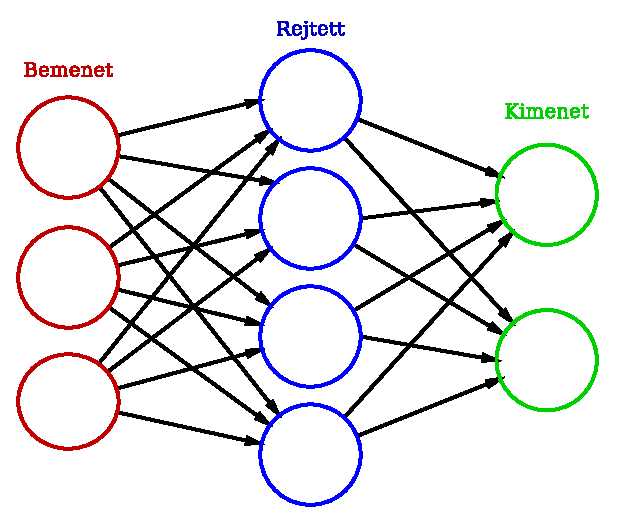
\includegraphics[width=0.3\columnwidth]{fig/neural_network}
	\caption{neurális hálózat réteges szerkezete \footnotesize forrás: en.wikipedia.org/wiki/Artificial\_neural\_network}
	\label{fig:neuralNet}
\end{figure}

A \ref{fig:neuralNet} ábrán a csúcsok jelentik a neuronokat és az élek a szinapszisok, melyeken az ingerület vándorol. Egy hálózat 3 nagyobb részre tagolódik:
\begin{enumerate*}[label={\alph*)},font=\bfseries]
	\item bemeneti réteg
	\item rejtett rétegek
	\item kimeneti réteg.
\end{enumerate*}
A bemeneti réteg csúcsai legtöbbször az adatot reprezentáló konstansok jelentik, tehát az egy egyszerű vektor.
Egy neuronban két művelet történik: a bementek összegzése és egy aktiváló függvény kiértékelés. Az összegzést a felsőbb rétegből érkező jelekre elvégezzük:
\begin{displaymath}
	s = \sum_i{w_ix_i}+b = \vec{w}\cdot\vec{x} + b
\end{displaymath}
ahol $x_i$ a felső réteg i.-ik neuronjának kimenete, $w_i$ az i.-ik neuron szinapszisához tartozó súly, mellyel a szinapszis "erősségét" határozzuk meg. Az "s" összeghez hozzáadunk még egy $b$  büntetőtagot, ami neuron aktiválási küszöbe lesz.
Az aktivációs függvény adja a neurális hálózat kimenetét, melynek paramétere $s$.
A neurális hálózatok fejlesztésekor sokféle függvényt találtak alkalmasnak aktivációs függvény gyanánt. Közös jellemzőjük, hogy inflexiós pontjuk $x=0$ helyen van, illetve 0-ban nem deriválható függvények esetén a töréspont esik ide.

A szemléletesség kedvéért tekintsünk meg az egyrétegű perceptront, vagyis egy egyetlen rétegből álló neurális hálózatot $k$ darab neuronnal. A bemenet legyen az $\vec{x}=(x_1,\dots,x_n)$ vektor. A szinapszisok súlyait a $W=\{w_{ij}:i=1\dots n,j=1\dots k\}$  mátrix ($\vec{w}_i$ az i. bemeneti adatból kiinduló szinapszisokhoz tartozó súlyok vektora lesz), a neuronok  büntetőtagját a $\vec{b}=(b_1,\dots,b_k)$ tartalmazza. Az aktivációs függvény $f$. A hálózat kimenetét, vagyis a  $\vec{y}=(y_1,\dots,y_k)$ elemeit megkapjuk a következőképpen:
\begin{displaymath}
	y_j = f(\vec{w}_i\cdot\vec{x}+b_j)
\end{displaymath}

A fentiekből látszik, hogy a hálózat tervezésénél annak négy tulajdonságát kell meghatároznunk:
\begin{enumerate*}
	\item a rétegek és azok neuronjainak számát
	\item a neuronok aktivációs függvényét (rétegenként egy típusú függvény az összes neuronra)
	\item a szinapszisok súlyát ($W=(\vec{w_1},\cdots\vec{W_n})$)
	\item a neuronok aktiválási küszöbét ($\vec{b}$).
\end{enumerate*}
Minden réteghez külön $W$ mátrixot és $\vec{b}$ vektort kell meghatározni. \textbf{Az egyszerűség kedvéért néha az egy réteghez tartozó $W$-t és $\vec{b}$-t együttesen nevezik a réteg \emph{súlyainak}}. Ez nagyon sok külön meghatározandó változót jelent, tehát csak az 1. és 2. tulajdonság meghatározása elvárható. Kell egy algoritmus, mellyel az egész hálózathoz tartozó paraméterek sokasága -- vagyis minden réteg súlyának paraméterei -- meghatározható.


\section{Deep Learning}
%A Deep Learning-ről szerzett tudásom javát F. Cholett könyvéből\cite{chollet} szereztem, melynek a témához kapcsolódó részleteit alább bemutatom.
Chollet könyvében részletesen kifejti mit is értünk \emph{Deep Learning} alatt, hogyan kapcsolódik a gépi tanulás fogalmához.\cite{chollet}

A gépi taunlás egy teljesen más programozási paradigmát jelent, ugyanis a klasszikus programozás során a feldolgozandó adatokhoz a programozó adja az adat feldolgozásának szabályait, amit végig követve a gép kiszámítja a kívánt eredményt. Ezzel szemben a gépi tanulás során a programozó az adathoz  a kívánt eredményt adja meg, amiből a gép felállítja a megoldáshoz vezető szabályokat.%\cite{Chollet}

A Deep Learning más néven a mély tanulás a gépi tanulás egy fajtája. Chollet szerint a név arra utal, hogy a kezdeti adaton több transzformációt végrehajtva egymás után egyre közelebb kerülünk egy olyan reprezentációhoz, ami megfelel a kívánalmainknak. Ezzel kontrasztban beszélhetünk sekély tanulásról, amikor kevés, egy vagy két transzformáció után kapjuk meg az adat megfelelő reprezentációját.%\cite{Chollet}
A neurális hálózatok rétegeltsége adja a \emph{mélységet} a gépi tanulásban. Eredeti elgondolás szerint minden egyes neuron-réteg egyre összetettebb tulajdonságokat ismer fel a bemeneti adatból. Valójában a rétegenkénti transzformációk egyre kisebb összetettségű hipotézis térbe visznek át, a reprezentáció egyre kevesebb -- a felhasználó számára fölösleges -- információt tartalmaz. Minél több réteg van a hálózatban, annál \emph{mélyebb} a modell.

\begin{figure}[h]
	\centering
	\includegraphics[width=0.8\columnwidth]{fig/digit_classification.png}
	\caption{Írott szám hozzárendelése az ábrázolt számértékhez\cite{chollet}}
	\label{fig:digit_classification}
\end{figure}

Itt kapcsolódik össze a neurális hálózat és a mély tanulás. Az \ref{sect:neuralNetworkTheory} alfejezetben kifejtettem, hogy a neurális hálózat szinapszisainak paraméterezéséért felelős $W$ mátrixok és a neuronok küszöbszintjének állítására szolgáló $\vec{b}$ vektorok összes koordinátájának száma hatalmas lehet, --~alkalmazástól függően több százezer, akár millió, egymástól független változóról beszélünk~-- tehát beállításukhoz valamilyen algoritmusra van szükség. Ezért a neurális hálózatok másik komponense, egy tanulási algoritmus, mely beállítja ezen paramétereket. Négy  megközelítés létezik, amikor gépi tanulásról van szó.

\emph{Ellenőrzött tanulás} során a neurális hálózatnak felcímkézett adatokat adunk meg, tehát olyan $y$ értéket  rendelünk az $x$ mintákhoz, amilyet szeretnénk, hogy a hálózat produkáljon. Ezen $z=(x,y)$ összerendezések halmazát \emph{tanítókészletnek} hívjuk. A hálózat leképezi az adatot a meghatározott reprezentációvá. A tanuló algoritmus ebből és a címkéből egy \emph{veszteség függvény} kiszámításával meghatározza, hogy mekkora az eltérés, a valamilyen értelemben vett távolság a kapott és az elvárt eredmény között. Ez alapján frissíti a $W$ mátrixot és $\vec{b}$ vektorokat.

\emph{Ellenőrizetlen tanulás}, mely során az adatokat nem címkézzük fel, hanem arra vagyunk kíváncsiak, hogy miféle összefüggések állnak fenn közöttük. Ezt a módszert adatbányászat során alkalmazzák. 

Az \emph{Önellenőrzött tanulás} hasonló az ellenőrzötthöz, azonban az adatok felcímkézését nem emberi erővel végezzük, hanem az adatokból állítjuk elő valamilyen heurisztikát felhasználva. Egyik alkalmazási területe az autóenkóderek tanítása.

A \emph{Megerősítéses tanulás} egy újfajta megközelítése a neurális hálózatok alkalmazásának. Ennél a metodikánál a hálózatot egy ágens alkalmazza, így a hálózat bemenete az ágens által megfigyelt környezet a kimenete pedig valamilyen cselekedet, beavatkozás és tanítás során az ágens igyekszik valamilyen környezetbeli értéket maximalizálni. Gyakori alkalmazás valamilyen játékot játszó ágens, ahol azt tanulja, adott helyzetekre milyen reakcióval tudja maximalizálni játékbeli pontszámát.
Vizsgálódásomat az \emph{ellenőrzött tanulásra} korlátoztam, így a továbbiakban ennek tükrében folytatom dolgozatomat.

\section{Függvények, algoritmusok}\label{sec:fuggvenyek-algoritmusok}
Az alábbiakban szeretném megfogalmazni a neurális hálózatokban alkalmazott tipikus függvényeket és algoritmusokat.

\subsection{Neuronok aktivációs függvényei}
Mint korábban kifejtettem minden neuron kimenete egy függvény kiértékelése, melynek paramétere a bemenetek súlyozott összege. Ezt a függvényt hívjuk aktivációs függvénynek. 

\paragraph{A szigmoid függvény}
Az utolsó, kimeneti neuronok rétegének aktivációs függvényeként alkalmazzuk, ahol a várt eredmény egyetlen valószínűségi érték. Ez bináris osztályozási problémák esetén alkalmazandó, tehát a program célja, hogy egy bemeneti adatról eldöntse, hogy az egy bizonyos kategóriába esik-e vagy sem, illetve erről mekkora "magabiztossággal" döntött.
\begin{equation}
	\sigma(x)= \frac{1}{1+e^{-x}}
	\label{eq:sigmoid}
\end{equation}\

\paragraph{A softmax függvény}
A kimeneti réteg aktivációs függvénye. $D$ dimenziójú $x$ vektorok koordinátáit normalizálja, másként fogalmazva egy tetszőleges $D$ elemű szám n-est azon $D$ elemű n-esek halmazába képezi, melyek elemeinek összege 1. Így tehát a $x$ koordinátái egy diszkrét valószínűségi eloszlás értékkészlete.\cite{wiki:softmax}
\begin{equation}
\sigma(x_i)=\frac{e^{x_i}}{\sum_{j=1}^{D}e^{x_i}},\quad i = 1,\dots,D
\label{eq:softmax}
\end{equation}
Éppen ezért többosztályos problémáknál használatos.A hálózat egy mintára adott válasza annak a diszkrét valószínűségi változónak az eloszlása, mely a minta egy adott kategóriába tartozásának a valószínűségét adja meg.

\paragraph{ReLu}
Teljes néven \emph{rectified linear unit} függvény vagy közismerten rámpafüggvény a rejtett neuron rétegek aktivációs értéke szokott lenni. Először 2011-ben mutatták be, hogy hatékonyabban taníthatóak a neurális hálózatok, mintha csak szigmoid függvényt használnánk neuronok aktivációs függvényeként.\cite{wiki:relu}
\begin{equation}
	f(x) = max\{0,x\}
	\label{eq:relu}
\end{equation}

\begin{figure}[h]
	\centering
	\begin{subfigure}[b]{0.3\textwidth}
		\def\svgwidth{0.5\columnwidth}
		\input{fig/Logistic-curve.pdf_tex}
		\caption{Szigmoid függvény}
		\label{fig:sigmoid}
	\end{subfigure}
	~
	\begin{subfigure}[b]{0.3\textwidth}
		\def\svgwidth{0.5\columnwidth}
		\input{fig/Ramp_function.pdf_tex}
		\caption{ReLu függvény}
	\end{subfigure}
	\caption{Aktivációs függvények grafikonja}
\end{figure}

\subsection{Veszteség függvények}
A neurális hálózat tanításához szükséges meghatároznunk egy $c(\vec{y},\vec{y'})$ veszteségfüggvényt, mely megadja a hálózat kimenetének eltérését az elvárt eredményhez képest adott súlyok mellett. Ezt az eltérést egy skalárértékként képezi le. Tanítás során ezt a függvényt kell minimalizálni.
%Formálisan egy $c:W\times B \mapsto \mathbb{R}^+$ függvény, $W,B$, a súlyokat és  büntetőtagokat egybefogó vektorok halmaza. Ezen többváltozós függvény képe a \emph{veszteségfelület}.

\paragraph[MSE]{Átlagos négyzetes hiba}\label{par:mse}
Többosztályos problémánál a neurális hálózat egy valószínűségi változó eloszlása az összes osztályon. $\vec{y}$ vektor a hálózat válasza a $\vec{x}$ bemenetre, $\vec{y'}$ pedig a kívánt kimenet vektora --~egy egységvektor, melynek 1 értékű koordinátája reprezentálja a megfelelő osztályt. Erre az esetre olyan veszteségfüggvényt alkalmazhatunk mely ekvivalens a $(\vec{x},\vec{y})\in Z$ tanítási készletből számított $MSE$ átlagos négyzetes hibáinak átlagával.\cite{nielsen2015}
\begin{align*}
	MSE(\vec{y},\vec{y'}) = \frac{1}{n}\sum_{i=1}^{n} (y_i - y'_i)^2\\
	C(w,b) \equiv \frac{1}{2m}\sum_{j=1}^{m} MSE(\vec{y}_j,\vec{y'}_j)\\
\end{align*}
A fenti egyenletekben n az kimeneti vektor dimenziója, m a tanító minták száma.
Chollet szerint osztályozási problémánál érdemes kereszt-entrópiát veszteségfüggvényként alkalmazni az átlagos négyzetes hiba helyett.\cite{chollet}
	%
	%\begin{displaymath}
	%	C(w,b)\equiv\frac{1}{2n}\sum_x\|y-y'\|^2\quad\footnote{forrás\cite{Nielsen2015}}
	%\end{displaymath}
%TODO nézd át

\paragraph{Kereszt-entrópia}
Osztályozási feladatoknál olyan módszert használhatunk a veszteség  vagy hiba érték számításához, melynél az $\vec{y}$ és $\vec{y'}$  kereszt entrópiáját határozzuk meg. Ilyen jellegű feladatoknál az említett vektorok valószínűségi eloszlások.
\begin{displaymath}
	H(y,y')= -\sum_{x\in \mathcal{X}}y(x)\log y'(x)
\end{displaymath}
A mély tanuláshoz használt keretrendszereknél gyakran másként implementálják a kereszt-entrópiát kétosztályos és többosztályos esetre. Ezekre az implementációkra \emph{bináris kereszt-entrópia} és \emph{kategorikus kereszt-entrópia} néven hivatkoznak.

\subsection{A hálózat tanító algoritmusai: az optimalizálók}
Korábban említettem, hogy egy neurális hálózat tanításán azt az eljárást értjük, amely során a hálózat paramétereit változtatjuk. Neurális hálózatoknál gradienscsökkentésen alapuló technikákat alkalmazunk. %A módszer alapját az az elképzelés adja, hogy  meghatározunk egy $C(\vec{w}_1,b_1,\dots,\vec{w}_L,b_L)$ függvényt, mely a hálózat összes paramétere alapján meghatároz egy $E$ hibaértéket, ami a tanítási folyamat egy ciklusa során kapott veszteségértékek átlaga.
A módszer megértéséhez, most tekintsünk úgy a költségre, mint a hálózat konfigurációjának jóságát értékelő függvényre.
$$ C(\vec{w}_1,b_1,\dots,\vec{w}_L,b_L) $$
Ezen függvény képe egy úgymond \emph{hibafelület}, melynek megkeressük  minimum helyeit tanítás során. Gyakorlatban nem kivitelezhető a globális minimum meghatározása, és lokális minimumok keresését is iteratív módszerekkel célszerű végezni. Többváltozós függvények esetén a gradiens vektor ellentettje ($-\nabla f$) segítségével meghatározható, hogy adott pontban -- azaz megadott függvényparaméterek esetén -- a paramétereket milyen mértékben változtassuk, hogy a függvény kimeneti értékét a legdrasztikusabb mértékben csökkentsük.
Belátható, hogy $C$ ekvivalens a $c$-k átlagával.
\begin{align*}
	\frac{1}{n}\sum_{i=1}^{n}c(y_i,y'_i) \equiv C(\vec{w}_1,b_1,\dots,\vec{w}_L,b_L)\\
\end{align*}
%TODO konzultálj ezzel kapcsolatban

A gradienscsökkentés naiv megközelítése pedig a következő:
\begin{align*}
	\vec{W_i}=(\vec{w_i}_1,b_{i1},\dots\vec{w_i}_L,b_{iL})\\
	\vec{W_{i+1}} = \vec{W_i} - \nabla C(\vec{W_i})
\end{align*}
Ahol $\vec{W_i}$ a tanítás i-edik ciklusában az $L$ rétegű hálózat összes paraméterének vektora.

\begin{figure}[h]
	\centering
	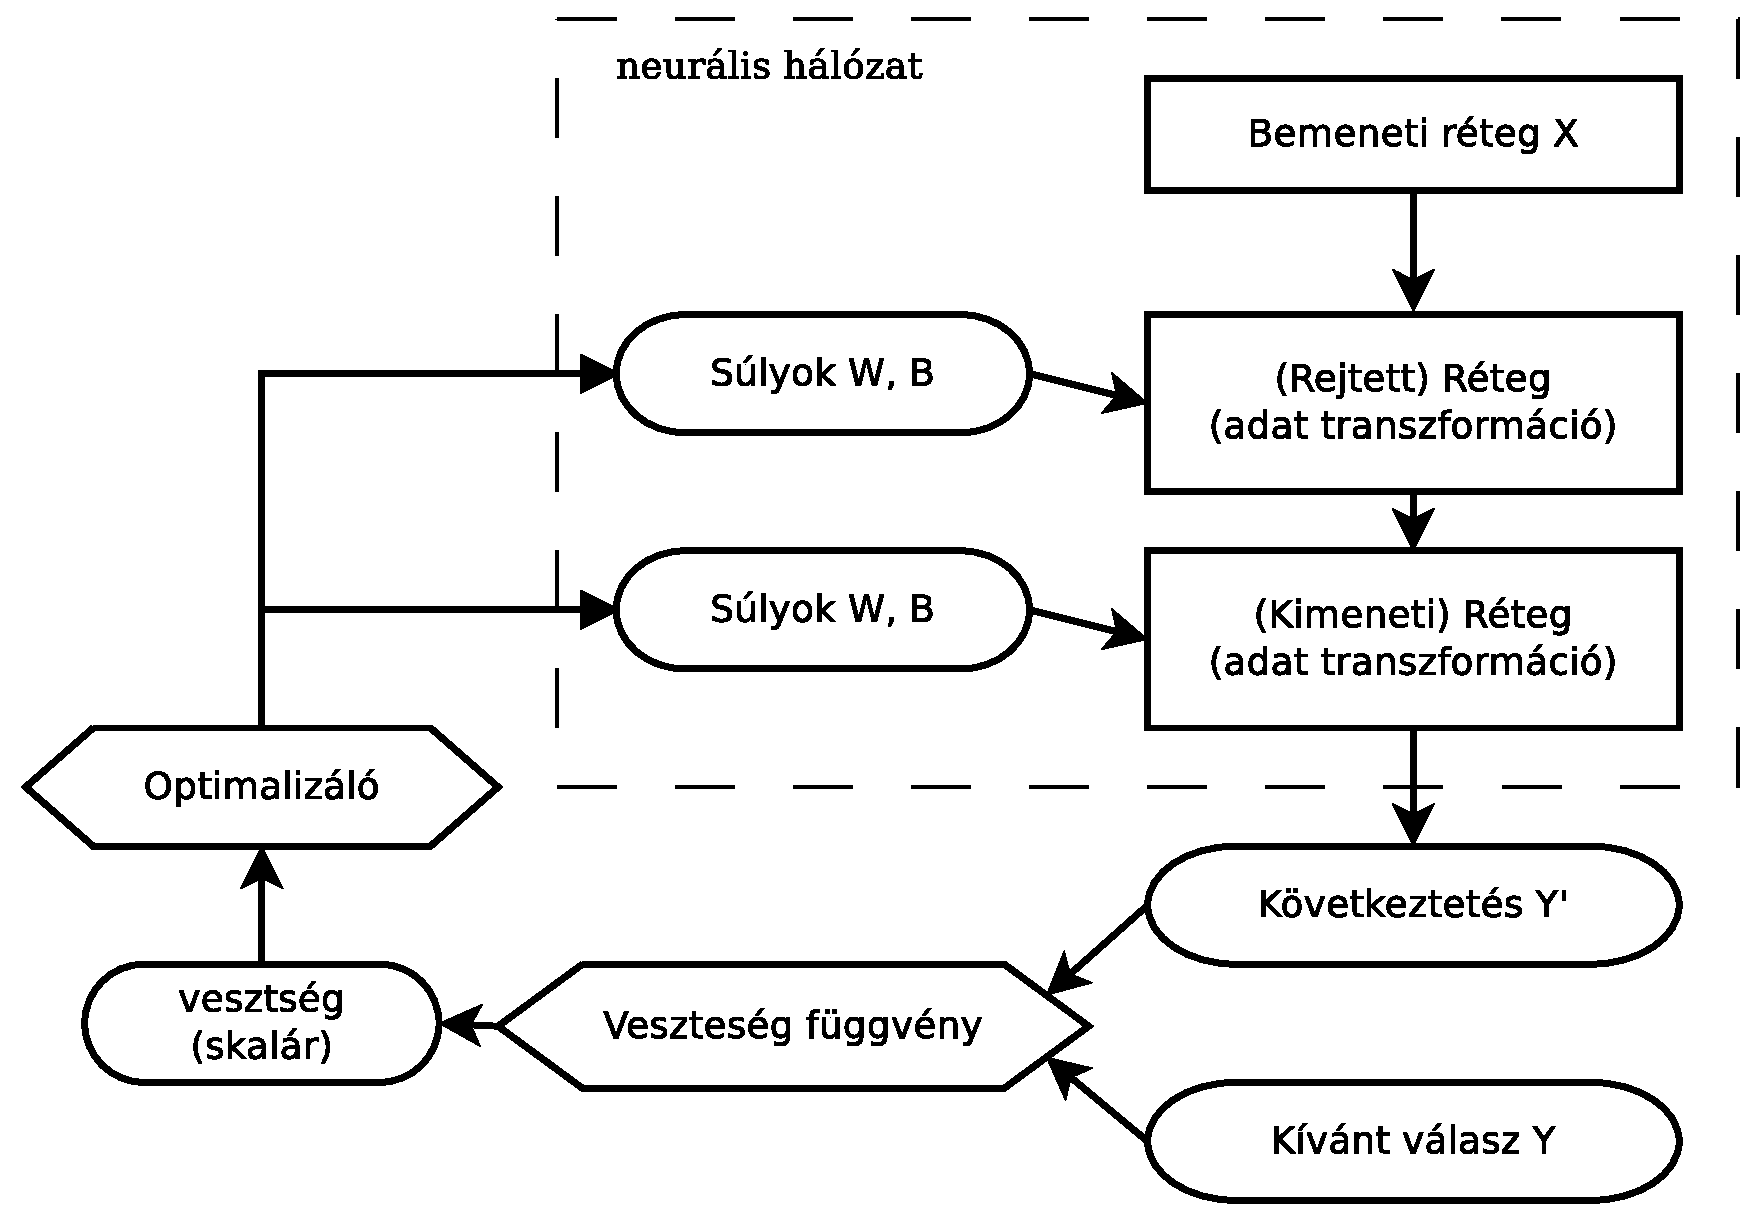
\includegraphics[width=0.7\linewidth]{fig/DNN_dia}
	\caption{A neurális hálózat tanításának folyamata}
	\label{fig:dnn}
\end{figure}

A tanítási folyamat iterációit \emph{eposzoknak} (angolul: epoch) nevezi a szakirodalom. Minden eposzban az optimalizáló hatására a kimeneti hiba csökken, a hálózat \emph{következtetése} egyre közelebb kerül az elvárthoz. 

\paragraph[SGD]{Sztochasztikus gradienscsökkentés}
A naiv megközelítést alapul véve meghatározunk egy $\eta$ tanítás sebességet (angolul: learning rate), mellyel azt befolyásoljuk, hogy egy eposzban a hálózat paramétereit mekkora mértékben változtatjuk. A tanítási sebesség az optimalizálók egy másik paramétere, tehát más eljárás esetén is alkalmazzuk valamilyen formában.
\begin{displaymath}
\vec{W_{i+1}} = \vec{W_i} - \eta\nabla C(\vec{W_i})
\end{displaymath}
Ezen paraméter változtatásánál fontolóra kell vennünk két tényezőt. Nagy tanítási sebesség gyorsabb gradiens csökkenést eredményez, ugyanakkor az elmozdulás a hibafelületen nagy kitérésekkel történik a minimumpont irányába. Túl kicsi tanítási sebességgel -- azon túl, hogy megnövekszik az eposzok szám --  ugyanakkor az optimalizálás "beragadhat" egy kedvezőtlen lokális minimum helyen.

\paragraph[RMSprop]{négzetes közép visszaterjesztése}
%RMSprop -> Root Mean Square propagation
Konstans tanulási rátát nehezen lehet jól megválasztani, ezért olyan eljárásokat dolgoztak ki, ahol ezen érték adaptálódik a tanítási folyamat során, hogy kiküszöbölje az előző bekezdésben említett nagy kitéréssel történő konvergenciát és a "beragadást". Az egyik ilyen módszer az, hogy a tanulási rátát elosztjuk az előző ciklusokban számított gradiensek nagyságának négyzetes közepével.
$$ v(w,y) = \gamma v(w,y-1) +(1-\gamma)(\nabla C(W_i))^2 $$
Ahol $\gamma$ az ún. felejtési tényező amivel szabályozhatjuk, hogy mekkora befolyása legyen az újabb gradienseknek.\\
A hálózat paramétereit a következőképpen frissítjük:
$$ W_{i+1} = W_i - \frac{\eta}{\sqrt{v(w_,y)}} \nabla C(W_i) $$
\\
Tanítás során a veszteségfüggvény sztochasztikusan konvergál a nullához és ezzel együtt a hálózat egyre pontosabban következtet a tanító készlet adataiból. A tapasztalat azonban az, hogy ez nem feltétlenül igaz más, a tanítás során nem használt adatokra, sőt elérkezhet a hálózat egy olyan állapotba, amikor a használat közben rosszabbul teljesít, mint a tanítás végén. Ilyenkor a hálózat specializálódik a tanító adathalmazra. Ezt a jelenséget, amikor a hálózat jobban következtet a tanítás során használt adathalmazon \emph{túlilleszkedésnek} nevezzük és \emph{alul-illeszkedésnek} azt, mikor a hálózat nem elég pontos, más szóval túl kevés tanítási cikluson esett még át. Hogy a hálózat a hipotézis térből a megfelelő függvények -- nem törekszünk az adatok egy tökéletes leképezésére -- valamelyikét modellezze, szükséges a tanítást felügyelni, hogy az ne illeszkedjen se túl, se alul.
A gyakorlatban ezért felügyeljük a tanítási folyamatot, és az optimalizálás minden ciklusában a hálózatnak egy külön validálásra szánt tanítókészletet adunk, és ezekre nem optimalizáljuk a hálózatot. Ezután össze tudjuk hasonlítani, hogy változik a hálózat hibája a tanító és validáló adatok mellett. Ennek tükrében abban a ciklusban ér el a hálózat a jól illesztett állapotot, amelyben a validációs veszteség érték eléri a minimumot.

\subsubsection{Regresszió optimalizálás}
%A bemeneti adatok tulajdonság szerinti normalizálása: x-átlag(x)/szórás(x) $$ s = \sqrt{\frac{1}{n-1}\sum_{i=1}^{n}(x_i - \bar{x})^2} $$
%
Osztályozási problémákon túl a mesterséges neurális hálózatok felhasználhatóak regresszióanalízisre. Ilyen feladatra tervezett hálózat kimeneti rétegének neuronjai aktivációs függvény nélküliek, tehát lineárisan képezik le a bemenetüket. Erre a kézenfekvő magyarázat, hogy a várt eredmény egy széles skálán mozoghat és bárminemű aktivációs függvény alkalmazása lekorlátozza az kimeneti adatok halmazát. Természetesen a többi réteg esetében alkalmazunk aktivációs függvényeket. Tanítás során az átlagos négyzetes hibafüggvényt --~amiről a \ref{par:mse}~bekezdésben már kitértem~-- alkalmazzuk veszteségfüggvény gyanánt. A hálózat pontosságának mérésére érdemes kiszámolni a hálózat következtetésének és az elvárt eredménynek átlagos abszolút eltérését, mint metrikát. A gyakorlatban a regressziószámítás sok változó skálán mozgó értékkel történik. A széles tartományon mozgó adatokon a hálózat nehezebben tanul, ezért a gyakorlatban érdemes a bemeneti adatokat normalizálni:
$$ s = \sqrt{\frac{1}{n-1}\sum_{i=1}^{n}(x_i - \bar{x})^2} $$
ahol $x$ a bemenő adathalmaz egy jellemzőjének egyetlen mintapontja, $n$ az egy jellemzőhöz tartozó minták száma, $\bar{x}$ pedig a minták átlaga.
Regressziószámítás a statisztikai alkalmazáson túl objektum detektálási feladatnál is felmerül: az objektumhatároló keretekhez tartozó vektorokat is többváltozós regresszióanalízissel határozhatjuk meg.
%TODO konzultálj
%-------------------------------------------------------------------------------
\chapter{Mély tanuló alkalmazások fejlesztése}
%-------------------------------------------------------------------------------
% TODO: Mélytanulásos keretrendszerek bemutatása általánosságban (mire jók, stb...)
A mély tanulás, azon belül is a mesterséges neurális hálózatok gyors fejlődősét és részben népszerűségét a hozzá készített programozási keretrendszereknek köszönheti, melyek java szabad hozzáférésű. Ezek a keretrendszerek arra hivatottak, hogy támogassák a neurális hálózatok fejlesztését új programozási módszertant adva. Már létező programozási nyelvekre épülnek, leginkább python-ra. Ezekben a keretrendszerekben egyszerűen implementálhatunk neurális hálózatokat úgy, hogy egyfajta nyelvi eszközkészletet adnak a hálózat definiálására.

\section{TensorFlow}

%TODO Nincs Befejezve
\section{Keras}

A Keras egy python nyelven írt programkönyvtár, vagy ahogy önmagát hívja ''magas szintű neurális hálózat API''\cite{web:Keras}. Érdekessége, hogy más olyan keretrendszerekkel együttesen használható, amelyek a Keras-hoz hasonlóan magas absztrakciós szinten biztosítják a hálózatok implementálását, mint például a TensorFlow. A Keras-ról szerzett tudásom javát Chollet könyvéből és a keretrendszer dokumentációjából szereztem.\cite{Chollet}\cite{web:Keras}.

\subsection{Neurális hálózat definiálása}

Keras-ban egy neurális hálózatot \emph{model}-nek hívunk (gyakran máshol is így neveznek egy konkrét neurális hálózatot). Egy \emph{model} létrehozásához a \verb|Keras.models| modulban definiált metódusokkal lehetséges. A keretrendszerben az adatokat tenzorokként kell reprezentálnunk, ezért érdemes a \emph{numpy}\footnote{lásd:\url{https://numpy.org/}} nevű python csomaggal együtt használni. A keretrendszer tetszőleges alakú tenzorokat képes kezelni, tehát nincs megkötés arra vonatkozóan, hogy egy réteg bemenete vektor, mátrix vagy kiterjedtebb struktúrában -- magasabb dimenziójú tenzorban -- szerepeljen. A következő kódokban szeretném szemléltetni a Keras használatának módját.

A \ref{lst:defLayers} kód egy két rétegből álló neurális hálózat definiálását mutatja be.
\begin{minipage}{\linewidth}
\begin{lstlisting}[language=Python, caption=Neurális hálózat rétegeinek definiálása]
from keras import models
from keras import layers

network = models.Sequential()
network.add(layers.Dense(32, activation='relu', input_shape=(784,)))
network.add(layers.Dense(10, activation='softmax'))
\end{lstlisting}\label{lst:defLayers}
\end{minipage}
Ezen lista 4. sorában inicializáljuk a hálózatot, az utána következő sorokban új neuron rétegeket adunk a hálózathoz.Keras-ban különböző előre definiált rétegkapcsolatok vannak. Itt a \verb|layers.Dense| osztály egy sűrűn kapcsolt réteget implementál. %TODO sürün kapcsolt réteg definíciója
A réteg bemenetként $28 *28 = 784$ elemű vektorokból álló mátrixot tud fogadni, másik dimenziója nem meghatározott. Ez a kötegelt adatfeldolgozás szempontjából fontos, tehát a bemeneti vektorok folyamát egyik dimenziójában nem meghatározott méretű tenzorral definiáljuk. A réteg kimenete egy 32 dimenziós vektor. A következő rétegnél nem adtuk meg a bemenet méretét, a keretrendszerben ez implicit módon rendelődik a réteghez. 

Mindkét réteghez tartozik egy \emph{activation} paraméter, mely string típus kell legyen, és a réteg neuronjaihoz tartozó aktivációs függvényt adja meg. A példában a \verb|'relu'| és \verb|'softmax'| string a \ref{sec:fuggvenyek-algoritmusok} fejezet \eqref{eq:relu} és \eqref{eq:softmax} függvényére utal, azaz ezen bemeneti paraméterek esetén olyan \verb|Dense| objektum jön létre, mely ilyen aktivációs függvényekkel rendelkező neuron réteget valósít meg.

A \verb|Keras.layers| modulban A \verb|Dense| osztályon kívül implementálva vannak konvolúciós, összefésülő, zaj, stb. rétegek, melyek a fenti módon tetszés szerint egymásra szervezhetőek a keretrendszerben, így szinte tetszőleges hálózat alakítható ki.

\subsection{Hálózat betanítása és következtetés futtatása}

A megalkotott hálózatot a \verb|network| objektum definiálja. Hogy tanítható legyen el kell látni egy optimizálóval és egy veszteségfüggvénnyel, melyek együtt adják a hálózatot betanító algoritmust. A \verb|compile()| metódus ,,összerakja'' a neurális hálózatot a betanítóval, a \verb|fit()| pedig elvégzi a tanítást, és \emph{epoch}-ok számának megfelelő méretű tömböket tartalmazó objektum referenciájával tér vissza, mely tömbökben össze vannak gyűjtve a veszteségfüggvény értékei és a felhasználói metrikák eposzonként. 

\begin{minipage}{\linewidth}
\begin{lstlisting}[language=Python,caption=Hálózat betanítása]
network.compile(optimizer = 'rmsprop',
loss = 'binary_crossentropy',
metrics = ['acc'])

history = network.fit(train_datas,
					train_labels,
					epochs=20,
					batch_size=512)
\end{lstlisting}\label{lst:fitNetwork}
\end{minipage}

A \verb|train_datas| és \verb|train_labels| a tanítókészletet alkotó minták és azok címkéi, a várt kimeneti értékek. Ezek elemszáma kötelezően meg kell egyezzen. A \emph{batch\_size} paraméterrel, ami az egy \emph{epoch}-ban egyszerre feldolgozandó adatokat jelenti. A betanítás végén a \verb|network| egy \emph{betanított}, a célfeladat megoldására felhasználható neurális hálózat lesz. Alkalmazásához a \verb|predict()|metódus használatos,mely a paraméterként megadott bemeneti adatokhoz tartozó predikciókkal tér vissza.
%TODO 
\begin{minipage}{\linewidth}
\begin{lstlisting}[language=Python, caption=Következtetés]
	result = network.predict(datas)
\end{lstlisting}
\end{minipage}

\subsection{Hatékonyságvizsgálat}


%TODO Nincs Befejezve
%-------------------------------------------------------------------------------
\chapter{Speciális platformok megjelenése}
%-------------------------------------------------------------------------------
\section{hybrid deep learning}
%TODO Nincs befejezve

\section{nGraph}
A most leírtak alapját az nGraph hivatalos dokumentációja adja\cite{web:ngraph_intro}.
Az nGraph az Intel\registeredlogo által fejlesztett programkönyvtár és egy futtatási környezet/fordító készlet melyet mély tanuló projektekhez.
Legszembetűnőbb tulajdonsága, hogy képes többféle hardver architektúrán futtatni és beépíthető számos keretrendszerbe.
Ezek azok a jellemzők, amiket kerestünk témavezetőmmel, hogy mély tanulást tudjunk végeztetni hatékonyan a \emph{HuSSar-on}. 
Ezen túlmenően a jövőbeli fejlesztések az iparban egyre jelentősebben igényelik, hogy a modern MI rendszerek skálázhatóak legyenek, mert egyrészt a neurális hálók egyre komplexebbé válnak, másrészt az általuk feldolgozott adatok mennyisége is rohamosan növekszik.

Jelenleg két bevett gyakorlat van a mély tanulás felgyorsítására:
\begin{enumerate}
	\item \textbf{Dedikált hardver tervezése a mély tanulással kapcsolatos számításokhoz} -- Sok vállalkozás tervez \emph{Alkalmazásspecifikus integrált áramköröket} (ASIC) neurális hálózatok betanítására és futtatására.
	\item \textbf{Szoftver optimalizáció} -- Programkönyvtárakat tartalmazó fejlesztési keretrendszerek fejlesztése, melyek képesek a hálózatokkal kapcsolatos számításokat több szálon, optimalizáltan futtatni. Az nGraph, mint fordító is egy ilyen megoldás.
\end{enumerate}

\subsection{Motiváció}
A mai legmodernebb szoftveres megoldás mély tanulásra az, ha integrálunk kernel könyvtárakat\footnote{Programkönyvtár, mely neurális hálókkal kapcsolatos elemi, \emph{mag} függvényeket tartalmazzák} mély tanulási keretrendszerekbe.
Ilyen integráció lehet például ha a Tensorflow keretrendszer alatt az Nvidia CuDNN könyvtárát használjuk.
A {kernel könyvtárak} egy adott célarchitektúrára optimalizált kernelekből és egyéb műveleti szintű optimalizálásokból állnak, ezekkel érve el teljesítménynövekedést.
Azonban a kernel könyvtáraknak három fő problémája van:
\begin{enumerate}
	\item Nem biztosítanak gráf szintű optimalizálást
	\item A keretrendszerek integrációja a {kernel könyvtárakkal} nem skálázható
	\item A szükséges lefordított kernel könyvtárak száma növekszik, ahogy új processzorok jelennek meg
\end{enumerate}
Az nGraph fordító megoldás az első két problémára, és a \emph{PlaidML}-el ötvözve kiküszöbölhető a harmadik probléma.
\subsection{Gráf szintű optimalizálás}
Az nGraph dokumentációjában áll egy példa arra vonatkozóan, hogyan lehet, hogy egy mély tanulási keretrendszer integrálva egy {kernel könyvtárral} a számításokat optimálisan végzi, mégis a számítási gráf a csúcsait alkotó műveletek szempontjából mégsem optimális.
\begin{figure}[!ht]
	\centering
	\includegraphics[width=0.9\textwidth]{kernel-problem-1.png}
	\caption{két optimalizálás módszer: konstans összehajtás és algebrai egyszerűsítés a gráfon. \protect \footnotemark}
	\label{fig:grafoptimalizalas}
\end{figure}
\footnotetext{forrás: \cite{web:ngraph_intro}}
A fenti ábra bemutatja, hogyan egyszerűsíthetünk az $A$,$B$ és $C$ tenzorokat feldolgozó, $ (A+B)*C $ tenzorműveletet végrehajtó számítási gráfon.
Fordítási időben megállapítható, hogy $B$ egy skalár konstans, így a \emph{konstans összehajtásnak} nevezett optimalizálás elvégezhető, és a 2 dimenziós vektorrá való kiterjesztés művelete elhagyható (helyette inkább közvetlenül létrehozunk egy $2\times2$ tenzort).
Ebben a példában $B=0$ skalár volt, így a belőle létrejött tenzor egy nullmátrix, így az semleges a kifejezés kiértékelésének szempontjából.
\emph{Algebrai egyszerűsítést} végezve az $ (A+0)*C $ leegyszerűsíthető az $A*C$ kifejezésre, így összesen két csúccsal csökkentettük a gráfunkat.
Ez az optimalizáció tehát a számítási gráf szintjén lett elvégezve.
Így belátható, hogy a mély tanulási keretrendszerbe integrált kernel programkönyvtárak nem optimális futást végeznek, hiába a műveletek szintjén elért optimalizálás. 
\subsection{Skálázható keretrendszer integráció}
Ahogy gyarapodik a mély tanuláshoz használható gyorsítókártya architektúrák és keretrendszerek száma, a meglévő mély tanulást alkalmazó fejlesztési platformok bővítése egyre több munkát igényel és egyre nő a hibák megjelenésének a valószínűsége. Az integráció kapható készen, szakértő fejlesztőcsapatoknak kell implementálnia.
Minden új keretrendszert manuálisan kell integrálni a meglévő hardverek kernel könyvtárával és minden újonnan megjelenő hardvercsalád meghajtó programkönyvtárát be kell integrálni egyesével a meglévő keretrendszerekbe.
Ez a munka önmagában is hatalmasra tud nőni, de egy sok eszközből álló összeállítás nagyon törékeny és költséges a fenntartása.
Az nGraph úgy oldja meg ezt a problémát, hogy ún. \emph{hidakat} alkalmaz, amikkel integrálható valamelyik mély tanulási keretrendszerbe.
A híd megkapja a keretrendszerben megalkotott számítási gráfot vagy ahhoz hasonló struktúrát és átalakítja egy ún. \emph{közbenső reprezentációvá}\footnote{IR: Intermediate Representation}. Ezzel kaptunk egy egységes, platformfüggetlen számítási gráfot, így nem kell egy új programkönyvtárat beintegrálni minden egyes meglévő keretrendszer alá, elegendő csak az, hogy az nGraph-ban, mint programkönyvtárban implementált \emph{primitív műveleteket} támogassa az új programkönyvtár.
\subsection{Növekvő kernel szám}
Egy kernel könyvtár integrálása egyszerre több mély tanulási keretrendszerrel nehéz feladat és egyre komplexebbé válik, ahogy növekszik az optimális teljesítményhez szükséges kernelek száma.
Régen a mély tanulással kapcsolatos kutatások egy kis számú \emph{primitív} számítást használtak, mint a konvolúció, általános mátrixszorzás, stb. Az MI kutatás előrehaladtával és az ipari mély tanuló alkalmazások továbbfejlesztésével, a szükséges kernelek száma (k) exponenciálisan nő.
Ez a szám a processzor architektúrák számán (h), adattípusokon (t), műveleteken (p) és az egyes paraméterek számosságán (p) alapul ($ k = h \times t \times m \times p $).
\begin{table}[!ht]
	\centering
	\begin{tabular}{|c|c|c|c|}
		
		Hardver & Művelet & Adattípus & Paraméterek \\ 
		\hline
		CPU & konvolúció & 16 bites lebegőpontos & NCHW vagy NHWC \\ 
		
		GPU & MatMul & 32 bites lebegőpontos & 2D, 3D és 4D tenzorok \\ 
		
		FPGA & Normalizálás & 8 bites egész &  \dots \\ 
		
		\dots & \dots & \dots & \\
	\end{tabular} 
	\caption{Néhány példa, tényezőnként hányféle esetre kell külön fordítani  kernelt könyvtárt }
	\label{table:kernels}
\end{table}

Ezen probléma megoldásához jön képbe a PlaidML. Ez egy \emph{tenzor fordító}\footnotemark, mely azt célozza, hogy képes legyen neurális hálózatokat tanítani és futtatni bármilyen típusú hardveren. Más szavakkal segíti a magas szintű keretrendszerek (Keras, ONNX, nGraph) integrálni olyan ezsközökkel, melyekhez nincs meg a szükséges támogatás vagy a meglévő szoftverkészlet hozzájuk szigorúan linceszelt.\cite{github:PlaidML}\cite{web:PlaidML}
\footnotetext{Olyan fordító, melynek nyelve arra lett fejlesztve, hogy főleg tenzorműveleteket igénylő számításokat tudjunk hatékonyan programozni}

Az nGraph tehát integrálható a PlaidML-el. Elsősorban az nGraph a platform független IR-rel igyekszik orvolsoni a skálázható backend-el kapcsolatos kihívást. A PlaidML ezt megtámogatja azzal, hogy képes az IR-ből származó gráfokból LLVM, OpenCL, OpenGL, CUDA és Metal kódot generálni melyek a megfelelő hardveren futtathatóak. Így egy magas szintű keretrendszerben írt neurális háló lefordul Intel és AMD processzrokon valamint grafikus processzorokon, az nVidia processzorain, továbbá az Apple cég által feljelsztett eszközökön.

Az nGraph gráf szintű optimalizációját ráadásul kiegészíti automatikusan a PlaidML alacsonyabb szinten, ezzel teljesítmény növekedést érve el.

Összegzésül tehát az nGraph feldarabolja a neurális hálózathoz tartozó számítási gráfot processzor architektúrának megfelelően, majd ezen gráfokat a PlaidML lefordítja a megfelelő kódokra, melyeket aztán a célprocesszorokra lefordítunk és futtatunk.

%TODO ide még jöhetne egy nGraph használatát bemutató alfejezet 
\section{Myriad X és az Intel Neural Computer Stick 2}
%Motiváció: Valós idejű alkalmazások esetén szükséges az offline számítás -> GPU - lehetséges, de erőforrás igényes(áram és hűtés) és nagy méretű 
Ma az iparban mély tanulással működő modern alkalmazások nagy méretű és teljesítményű számítógépeket igényelnek. Erre az igényre válaszul felhő szolgáltatást nyújtó vállalatok külön platformot építettek ki. Az ilyen kliens-szerver architektúrájú gépi tanulás hatékony lehet, azonban a valós-idejű alkalmazásoknál és hordozható eszközökben történő felhasználásnál komoly hátrányt jelenthet a hálózati késleltetés. Hogy ilyen területeken is alkalmazható legyen a mély tanulás, hardvergyártók olyan kis energiafogyasztású \emph{alkalmazás-specifikus integrált áramkörök} fejlesztésére törekedtek, melyek képesek neurális hálózatokat hatékonyan futtatni. Ilyen az Intel által kifejlesztett Myriad X lapka is, melyet főleg \emph{gépi látáshoz} terveztek.

Maga a Myriad egy Videójel feldolgozó processzor széria, melynek 3. generációja a Myriad X architektúrája kiegészült egy úgynevezett \emph{Neural Compute Engine-el}, mely a betanított hálózatok futtatását hivatott gyorsítani. Ezzel együtt a lapka 16 darab 128-bit VLIW processzormagok, ún. SHAVE magot és 2,5MB 400GB/s sávszélességű memóriát tartalmaz. Számításokat 8bites egészek és 16bites lebegőpontos váltózókon tud végezni.\footnote{forrás: https://www.movidius.com/myriadx} 
% TODO Myriad X

A Myriad X kifejlesztésén túlmenően a vállalat tervezett egy gyorsítókártyát is ehhez a processzorhoz, melyet Neural Compute Stick (NCS) névvel forgalmaz. Az Intel kiadta a második verzióját az eszköznek  Neural Compute Stick 2 (NCS2) névvel és az első verziót nem forgalmazz már. Ezért a továbbiakban a leírtakat az NCS2-re kell érteni.
Az eszköz USB 3.0 -ás interfésszel rendelkezik, így sok gazdagéppel használható, többek között Raspberry Pi-vel is. Meghajtására az Intel OpenVINO eszközkészlete használható, melyet gépi látáson alapuló alkalmazások fejlesztésére készített a vállalat. Lehetőség van egy platformon több NCS2 modul együttes használatára, így egyszerűen növelhető a rendszer teljesítménye.
\begin{figure}[h]
	\centering
	\includegraphics[width=0.5\linewidth]{fig/NCS2-specs}\\
	\footnotesize forrás:https://software.intel.com/en-us/neural-compute-stick
	\caption{Neural Compute Stick 2 gyorsító} 
	\label{fig:ncs2-specs}
\end{figure}
%TODO Nincs Befejezve

\subsection{Az NCS2 használata OpenVINO keretrendszerben}
Az alábbiak alapját az Intel OpenVINO eszközkészletének dokumentációja adja.\cite{web:OpenVINO} A dokumentációban a felépített neurális hálózatokra modell néven hivatkoznak, amit most én is átveszek.

Az OpenVINO eszközkészlet alkalmas arra, hogy gyorsan készítsünk olyan alkalmazásokat, melyek valamilyen módon emulálják az emberi látást. Képesek vagyunk segítségével az NCS2-n kívül más Intel gyártmányú hardverrel dolgozni, például Intel CPU-n és integrált GPU-n. Továbbá népszerű keretrendszereket támogat, mint a TensorFlow, Caffe, MXNet vagy az ONNX. Az eszközkészlet komponensekei közül az alábbiakat emelném ki:
\begin{description}[noitemsep]
	\item[Inference Engine] python API, aminek segítségével különböző gyorsítókártyák megszólíthatók egységes módon.
	\item[Model Optimizer] parancssoros alkalmazás mentett modellek átkonvertálására. Ahhoz, hogy a különböző keretrendszerekben megalkotott modelleket egységesen tudja kezelni az Inference Engine, szükség van azok átkonvertálására egy platformfüggetlen struktúrába.
	\item[OpenCV] az OpenCV közösségi fejlesztésű verziójának Intel hardverekre fordított változata.
\end{description}

Az OpenVINO-val való munka folyamatának három fő lépése van:
\begin{enumerate*}[label={}, font=\bfseries]
	\item Betanított Neurális hálózat beszerzése;
	\item a hálózat átkonvertálása a Model Optimizer-rel;
	\item python szkript implementálása az Inference Engine-t tartalmazó modulokkal, melyben az átkonvertált fájlokat lefuttatjuk a célhardveren
\end{enumerate*}

\section{Google Edge TPU}
Az Intelhez hasonlóan a Google is tervezett célprocesszort és hozzá fejlesztő panelt, mély tanulást alkalmazó projektekhez. A Google Edge TPU-ról és a Coral USB Accelerator-ról a Heartbeat internetes magazinban megjelent cikkben értesültem.\cite{web:GoogleEdge} A Google TPU-ról szerzett ismereteim a wikipédia ,,Tensor Processing unit'' cikkéből szereztem.\cite{wiki:TPU}

\begin{figure*}[h]
	\centering
	\includegraphics[width=0.4\textwidth]{fig/penny-edge-tpu}\\
	\footnotesize forrás: https://cloud.google.com/edge-tpu/
	\caption{Edge TPU}
	\label{fig:EdgeTPU}
\end{figure*}
\begin{figure*}[h]
	\centering
	\includegraphics[width=0.4\textwidth]{fig/Coral_USBAccelerator}\quad
	\caption[Coral USB Accelerator]{Az Edge TPU-t építették az USB interfésszel ellátott Coral USB Accerlerator-ba.\cite{web:GoogleEdge}}
	\label{fig:coralusbaccelerator}
\end{figure*}


A Google a Tensor Processing Unit\texttrademark-ot, egy saját fejlesztésű alkalmazásspecifikus integrált áramkört használ a neurális hálózatokkal kapcsolatos számítások optimalizálására. Ezek lényegében mátrix műveletekre számítására fejlesztett processzorok CISC utasításkészlettel. Három generációt ért meg, az első még csak 8-bites egészeken tudott műveleteket végezni, azonban már a második generáció képes volt lebegőpontos számításokra is. A Tensor processing unit-okkal felszerelt gyorsítókártyákat a Google saját adatközpontjaiban használja főként és elérhetővé teszi őket a \emph{Google Cloud Platform} nevű szolgáltatásán keresztül. Nevéből adódóan a kártya architektúrája lehetővé teszi, hogy  tenzorműveletek tudjanak hatékonyan végrehajtani, utasításkészletük kifejezetten támogatja a neurális hálózatokat. Ilyen művelet a konvolúció és az \ref{sect:neuralNetworkTheory} alfejezetben tárgyalt aktváló függvények alkalmazása a mátrix szorzáson túl.

Az Edge TPU a cég szerverei által használt TPU-hoz viszonyítva kisebb méretben és energiafogyasztásban. Ugyan azt az igényt igyekszik kielégíteni, mint a korábban bemutatott Myriad X processzor. Azzal összehasonlítva viszont képes neurális hálózatok tanítására is korlátozott mértékben. Az Edge TPU részét képezi a Google Coral eszközkészletének, mellyel alternatívát nyújtanak a felhőalapú Cloud AI szolgáltatással szemben. A Coral különböző fajtájú hardvert nyújt a felhasználóknak, mindegyik központi eleme az Edge TPU. Az eszköz programozásához használható API-t az Edge TPU python könyvtár (\verb|edgetpu| python modul) valósítja meg, amely képes TensorFlow Lite-ban alkotott betanított neurális hálózatok futtatására. A könyvtár kulcsfontosságú interfészeit a következő osztályok képezik.Képosztályozási feladatokhoz a \verb|ClassificationEngine| használatos, vizuális objektumazonosításra a \verb|DetectionEngine|. Az \verb|ImprintingEngine| és \verb|SoftmaxRegression| az ún. \emph{transzfer tanuláshoz} alkalmazható, vagyis előre betanított hálózatok a feladatnak megfelelő újratanítását végezhetjük el vele.


\section{Új gyorsítók: Intel Nervana Neural Network Processor}

%TODO Nincs Befejezve

%-------------------------------------------------------------------------------
\chapter*{Összefoglalás}\addcontentsline{toc}{chapter}{Összefoglalás}
%-------------------------------------------------------------------------------
%\lipsum[1]
A gépi tanulás olyan területeken jelent meg melyek új kihívásokat szültek. A hardvergyártók kifejezetten deep learningre optimalizált megoldásokat kínálnak és a jövőbeli fejlesztések is ebbe az irányba mutatnak. Ezen dolgozatomban bemutatott, mély tanulásban használatos technológiákon látható, hogy egyre változatosabb deep learning rendszereket alapját tudják nyújtani. Olyan keretrendszerek születtek független fejlesztőcsapatok és a hardvergyártók jóvoltából, melyekkel gyorsan és hatékonyan végezhető mély tanuló alkalmazások fejlesztése. Ennek jóvoltából a mindennapi életben is megjelenik ez a technológia, és azon is túl a kutatásokban megjelenő nehezen megoldható számítási problémák váltak kivitelezhetővé. Ezen technológiákat felölelő szakterületek a munkaerőpiacon is igen keresetté válhatnak.

A hardveripar most is sok erőforrást fektet a gyakorlatban használt mesterséges neurális hálózatok hatalmas számítási igényének kielégítésére. Újabb és hatékonyabb eszközöket kínálnak erre a feladatra. Némelyikük a korábban bevált GPGPU architektúrák továbbfejlesztése, míg mások speciális, csakis kifejezetten deep learning architektúrák. Ezek az eszközök a több magos masszívan párhuzamos számításokra alapoznak, melyek jól alkalmazhatóak a neurális hálózatokon.

Ezzel párhuzamosan hibrid számítási rendszereket támogató keretrendszerek is készülnek, szintén a párhuzamos számítás modellre, azontúl az egyes architektúrák eltérő működésére alapozva. Ennek köszönhetően a deep learning alkalmazások változatos hardver architektúrákon futtathatóak, melyek a nyers erőn túl a számítások hatékony végrehajtásával érnek el teljesítménynövekedést. Az ilyen technológiák továbbá lehetőséget biztosítanak, hogy a felhasználók meglévő hardvereiket építsék be deep learning rendszerekbe. Ez a fejlesztési költségek szempontjából nagyon előnyös, ezért a jövőben várhatóan egyre több szerveren találkozhatunk tanuló vagy tanítható alkalmazásokkal.

A nagygépes világgal párhuzamosan megjelentek külön mély tanulásra specializált integrált áramkörök a hordozható és személyi eszközökön is. A Deep Learning így egy ,,kézzel fogható'' technológiává válik. Ez az irány elősegíti a valós idejű mély tanuló alkalmazások fejlesztését, mint például az önvezető járművek, intelligens gyártósorok, személyi applikációk vagy egyes orvosi alkalmazások. Úgy látszik a jövőben erre a szolgáltatók is számítanak: ezen speciális hardverek némelyike építőkövei lehetnek az ún. \emph{Edge Computing} modellnek: míg kezdetben a felhőszolgáltatásokat nyújtó vállalatok neurális hálózatai teljes egészében szervereiken futottak, mára kezd kibontakozni az az elképzelés, hogy ezeket a számításokat a felhasználóhoz egészen közel lehet vinni, így közel valós idejűek lehetnek a felhő alapú deep learning szolgáltatások is a jövőben.

A szakdolgozatom írása során rengeteg új ismeretre tettem szert. Igyekeztem a legmodernebb hardvereket és legújabb szoftverfejlesztéseket felkutatni. Így szembesültem azzal is, hogy ennek a szakterületnek csak felszínét vizsgáltam még. Ahhoz, hogy tényleg jó rálátásom legyen a jövőbeli fejlesztésekre, a gépi tanulással kapcsolatos ismereteimet mesterképzésben szeretném elmélyíteni.

Az nGraph lefordításának sikertelensége témavezetőm hibrid rendszerére nem tántorított el a korábban megfogalmazott terv kivitelezésétől. A keretrendszer élénk fejlesztését látva van esély rá, hogy a későbbiekben újból megkíséreljük lefordítani a HuSSarra, hogy öszevethessük az nGraph teljesítményét más hibrid rendszereken működő fordítókéval.
\clearpage

% irodalomjegyzék
%---Hagyományos---
%----------------------------------------------------------------------------
%Irodalomjegyzék
%----------------------------------------------------------------------------
\begin{thebibliography}{9}
%Könyvek,cikkek,tanulmányok
\bibitem{Chollet}
	François Chollet,
	\textbf{Deep Learning with Python},
	Manning Publications,
	2018.

\bibitem{neural2006}
	Altrichter Márta \& Horváth Gábor \& Pataki Béla \& Strausz György \& Takács Gábor \& Valyon József,
	\textbf{Neurális hálózatok},
	Panem,
	2006,
	[Szakkönyv],

\bibitem{mccullogh1943}
	McCulloch, W.S. \& Pitts, W.,
	\textbf{A Logical Calculus of Ideas Immanent in Nervous Activity},
	Bulletin of Mathematical Biophysics,
	1943,
	doi:10.1007/BF02478259.

\bibitem{Nielsen2015}
	Michael A. Nielsen,
	\textbf{Neural Networks and Deep Learning},
	Determination Press
	2015.
	\newline{\footnotesize\url{http://neuralnetworksanddeeplearning.com/}}
	[online, meglátogatva: 2019.~október~30.]
	
%adatforrások

%jogszabályok

%Kézikönyvek

\bibitem{web:PlaidML}
	\textbf{PlaidML -- Home},
	2019.~október~20.,
	Vertex.AI.,
	\newline{\footnotesize\url{vertexai-plaidml.readthedocs-hosted.com/en/stable/}}

\bibitem{web:ngraph_intro}
	\textbf{Introduction --- Documentation for the {nGraph} Library and Compiler stack},
	2019,
	\newline{\footnotesize\url{ngraph.nervanasys.com/docs/latest/introduction.html}}
	[meglátogatva: 2019.~október~08.]

\bibitem{web:OpenVINO}
	\textbf{OpenVINO\textsuperscript{\texttrademark}\space toolkit Documentation},
	2019,
	\newline{\footnotesize\url{docs.openvinotoolkit.org/2019_R3/index.html}}
	[meglátogatva: 2019.~november~4.]

%Internetes adatgyűjtés

\bibitem{web:GoogleEdge}
	\textbf{Edge TPU: Hands-On with Google’s Coral USB Accelerator},
	\newline{\footnotesize\url{heartbeat.fritz.ai/edge-tpu-google-coral-usb-accelerator-cf0d79c7ec56}}
	[meglátogatva: 2019.~október~23.]

\bibitem{web:Keras}
	\textbf{Keras Dokumentáció},
	\newline{\footnotesize\url{keras.io/}}
	[meglátogatva: 2019.~október~23.]

\bibitem{web:NNP}
	\textbf{Intel® Nervana™ Neural Network Processors},
	\newline{\footnotesize\url{www.intel.ai/nervana-nnp/}}
	[meglátogatva: 2019.~november~07.]

%\bibitem{web:Raoblog2019}
%	Naveen Rao,
%	\textbf{‘‘Accelerating with Purpose'' for AI everywhere},
%	2019,
%	\newline{\footnotesize\url{www.intel.ai/accelerating-for-ai/}}
%	[blog, meglátogatva: 2019.~November~07.]

%\bibitem{web:Raoblog2017}
%	Naveen Rao,
%	\textbf{Intel® Nervana™ Neural Network Processors (NNP) Redefine AI Silicon},
%	2017,
%	\newline{\footnotesize\url{www.intel.ai/intel-nervana-neural-network-processors-nnp-redefine-ai-silicon/}}
%	[blog, meglátogatva: 2019.~November~07.]

\bibitem{web:IntelNews2019}
	\textbf{At Hot Chips, Intel Pushes ‘AI Everywhere’},
	2019,
	\newline{\footnotesize\url{newsroom.intel.com/news/hot-chips-2019/}}
	[meglátogatva: 2019.~November~07.]

\bibitem{slide:nnpt}
	Andrew Yang,
	\textbf{Deep Learning Training At Scale	Spring Crest Deep Learning Accelerator (Intel® NervanaTM NNP-T)},
	2019,
	\newline{\footnotesize\url{www.slideshare.net/insideHPC/deep-learning-training-at-scale-spring-crest-deep-learning-accelerator/}}
	[letöltve: 2019.~november~07.]

\bibitem{yt:nnpt}
	Intel AI,
	\textbf{Introducing Intel Nervana Neural Network Processors for Training},
	2019,
	\newline{\footnotesize\url{www.youtube.com/watch?v=Wj4ifr3DDFg}}
	[megtekintve: 2019.~november~10.]

\bibitem{slide:nnpi}
	Ofri Wechsler \& Michael Behar \& Bharat Daga,
	\textbf{Spring Hill (NNP-I 1000) Intel’s Data Center Inference Chip},
	2019,
	\newline{\footnotesize\url{www.slideshare.net/insideHPC/spring-hill-nnpi-1000-intels-data-center-inference-chip/}}
	[letöltve: 2019.~november~07.]

\bibitem{yt:nnpi}
	Intel AI,
	\textbf{Introducing Intel Nervana Neural Network Processors for Inference},
	2019,
	\newline{\footnotesize\url{www.youtube.com/watch?v=fTMIjQePWog}}
	[megtekintve: 2019.~november~10.]

	%Github

\bibitem{github:nGraph}
	\textbf{NervanaSystems/ngraph: nGraph - open source C++ library, compiler and runtime for Deep Learning},
	GitHub repository,
	2019,
	\newline{\footnotesize\url{github.com/NervanaSystems/ngraph}}

\bibitem{github:PlaidML}
	\textbf{plaidml/plaidml: PlaidML is a framework for making deep learning work everywhere},
	GitHub repository,
	\newline{\footnotesize\url{github.com/plaidml/plaidml}}
	[meglátogatva: 2019.~október~20.]

	%Wikipedia

\bibitem{ wiki:constfold}
	\textbf{Constant folding --- {Wikipedia}{,} The Free Encyclopedia},
	2019,
	\newline{\footnotesize\url{en.wikipedia.org/w/index.php?title=Constant_folding&oldid=914455114}}
	[meglátogatva: 2019.~október~09.]
	
	\bibitem{wiki:plaidml}
	\textbf{PlaidML --- {Wikipedia}{,} The Free Encyclopedia},
	2019,
	\newline{\footnotesize\url{en.wikipedia.org/w/index.php?title=PlaidML&oldid=898300482}}
	[meglátogatva: 2019. október 5.]
	
	\bibitem{wiki:relu}
	\textbf{Rectifier (neural networks) --- {Wikipedia}{,} The Free Encyclopedia},
	2019,
	\newline{\footnotesize\url{ en.wikipedia.org/w/index.php?title=Rectifier_(neural_networks)&oldid=923288576}}
	[Meglátogatva: 2019.~október~29.]
	
	\bibitem{wiki:TPU}
	\textbf{Tensor processing unit --- {Wikipedia}{,} The Free Encyclopedia},
	2019,
	\newline{\footnotesize\url{en.wikipedia.org/w/index.php?title=Tensor_processing_unit&oldid=923241091}}
	[Meglátogatva: 2019. november 4.]

\end{thebibliography}
%---Biblatex---
%\bibliographystyle{tex/bibstyle}
%\bibliographystyle{plain}
%\bibliography{bib/bibliography}
%---Biblatex biblatex usepackage-al---
%\printbibliography[heading=bibintoc, title={Irodalomjegyzék}]

% függelék
%\include{tex/fuggelekek}

%%----------------------------------------------------------------------------
\chapter*{Köszönetnyilvánítás}\addcontentsline{toc}{chapter}{Köszönetnyilvánítás}
%----------------------------------------------------------------------------
Ezúton köszönöm témavezetőmnek biztatását amit a neurális hálózatokkal való ismerkedésem során nyújtott továbbá, hogy mindig számíthattam a segítéségére. A mély tanulás iránti lelkesedésével engem is átitatott, mely átsegített a nehézségeken. Nélküle talán sose ismerkedtem volna meg közelebbről ezzel a területtel. Szeretném továbbá megköszönni szüleimnek azt, hogy mellettem álltak, mikor szakterületet váltottam és támogatták egyetemi tanulmányaimat.

\end{document}